\documentclass[11pt,xcolor={svgnames},aspectratio=169,usepdftitle=false]{beamer}

% Add space in lists
\let\toneitemize\itemize
\let\ttwoitemize\enditemize
\renewenvironment{itemize}{\toneitemize\addtolength{\itemsep}{1.35\baselineskip}}{\ttwoitemize}

\let\toneenumer\enumerate
\let\ttwoenumer\endenumerate
\renewenvironment{enumerate}{\toneenumer\addtolength{\itemsep}{1.35\baselineskip}}{\ttwoenumer}

% Alert color
\setbeamercolor{alerted text}{fg=DarkOrange}

% Itemize w bullets
\setbeamertemplate{itemize items}{$\circ$}

% Font size of title
\setbeamerfont{title}{size=\huge}

% Transition section slides
\setbeamertemplate{section page}
{
    \begin{centering}
    \begin{beamercolorbox}[sep=12pt,center]{part title}
        \setbeamerfont{section title}{size=\huge}
        \usebeamerfont{section title}\insertsection\par
    \end{beamercolorbox}
    \end{centering}
}

%===========================================================
% Color specifications
%===========================================================
\definecolor{GreyishBlue}{HTML}{087E8B} 	% Headings color
\definecolor{CitationsBlue}{HTML}{2B6684} 	% Color for citations
\definecolor{LinksPink}{HTML}{ff0054}       % Color for links

% Template for syntax highlighting
\definecolor{BeigeBackground}{HTML}{fdf6e3}
\definecolor{BlueKeyWord}{HTML}{268bd2}

\setbeamercolor{palette primary}{bg=GreyishBlue,fg=white}
\setbeamercolor{palette secondary}{bg=GreyishBlue,fg=white}
\setbeamercolor{palette tertiary}{bg=GreyishBlue,fg=white}
\setbeamercolor{palette quaternary}{bg=GreyishBlue,fg=white}
\setbeamercolor{structure}{fg=GreyishBlue} % itemize, enumerate, etc
\setbeamercolor{section in toc}{fg=GreyishBlue} % TOC sections
\setbeamercolor{background canvas}{bg=white}
\setbeamercolor{button}{bg=white, fg=GreyishBlue}

%===========================================================
% Numeration in environments
%===========================================================
\setbeamertemplate{theorems}[numbered]
\setbeamertemplate{definitions}[numbered]
\setbeamertemplate{navigation symbols}{}
\setbeamertemplate{caption}[numbered]

\usepackage{appendixnumberbeamer}

%===========================================================
% Language and font settings
%===========================================================
\usepackage[english,activeacute]{babel} % Language
\usefonttheme{professionalfonts}		% Avoid overwriting fonts

\usepackage[sfdefault,light]{FiraSans}
\usepackage[utf8]{inputenc}				% Special symbols
\usepackage[T1]{fontenc}				% T1 Encoding of font

%===========================================================
% Math font settings
%===========================================================
\usepackage{mathpazo}					% Math font
\usepackage{amsmath,amsfonts,amssymb}	% Math symbols
\usepackage{dsfont}						% Math symbols like R for reals...

%===========================================================
% References' colors and PDF properties
%===========================================================
\usepackage{hyperref}
\hypersetup
{
    pdfauthor={Rafael Serrano Quintero},
    pdfsubject={Introduction to Matlab},
    colorlinks = {true},
    linkcolor = {GreyishBlue},
    citecolor = {LinksPink},
    urlcolor = {LinksPink},
    filecolor = {LinksPink}
}
%===========================================================
% Additional packages
%===========================================================
\usepackage{graphicx}
\usepackage{tikz}

\usepackage{longtable}
\usepackage{appendix}
\usepackage{marvosym}
\usepackage{enumerate} %For enumerating with letters with option [a)]
\usepackage{epstopdf}
\usepackage[round]{natbib}
% Change manually the color of the parenthesis
\bibpunct{\textcolor{CitationsBlue}{(}}{\textcolor{CitationsBlue}{)}}{,}{a}{}{;}

\usepackage[flushleft]{threeparttable}
\usepackage{booktabs}
\usepackage[super]{nth}
\usepackage{float}
\usepackage{caption}
\usepackage{subcaption}
\usepackage{multicol}

%========================================================================================
% Syntax highlighting for Matlab
%========================================================================================
\usepackage{fancyvrb}  %To reduce font size in verbatim environment
\usepackage{listings}


\lstloadlanguages{Matlab}%
\lstset{
    language=Matlab,
    basicstyle=\small\ttfamily,
    backgroundcolor=\color{BeigeBackground}, 
    breaklines=true,                 
    captionpos=b,                    
    commentstyle=\color{gray},   
    frame=none,
    keywordstyle=[1]\color{BlueKeyWord}\bfseries, % MATLAB functions bold and blue
    keywordstyle=[2]\color{Purple},  % MATLAB function arguments purple
    keywordstyle=[3]\color{Purple}\underbar,  % User functions underlined and blue      
    stringstyle=\color{Purple},   
    morekeywords={xlim,ylim,var,alpha,factorial,poissrnd,normpdf,normcdf,ones},
    %Put MATLAB function parameters here
    morekeywords=[2]{all, on, off, interp},
    morecomment=[s]{\%\{}{\%\}},
    numbers=left,                    
    numbersep=3pt,                   
    numberstyle=\tiny\color{black},
    rulecolor=\color{black},        
    showspaces=false,               
    showstringspaces=false,          
    showtabs=false,                  
    stepnumber=1,                    
    tabsize=2         
}

\newtheorem{exercise}{Exercise}
%===========================================================
% DOCUMENT
%===========================================================
\title{Introduction to Matlab}
\subtitle{Lesson 01 --- Preliminaries and Matlab Syntax}

\author{Rafael Serrano-Quintero}

\institute{Department of Economics \\ University of Barcelona}
\date{}

\AtBeginSection[]{\frame{\sectionpage}}
\AtBeginSubsection[]{\frame{\subsectionpage}}

\defbeamertemplate{section page}{mine}[1][]{%
  \begin{centering}
    {\usebeamerfont{section name}\usebeamercolor[fg]{section name}#1}
    \vskip1em\par
    \begin{beamercolorbox}[sep=12pt,center]{part title}
      \usebeamerfont{section title}\insertsection\par
    \end{beamercolorbox}
  \end{centering}
}

\defbeamertemplate{subsection page}{mine_sub}[1][]{%
  \begin{centering}
    {\usebeamerfont{subsection name}\usebeamercolor[fg]{subsection name}#1}
    \vskip1em\par
    \begin{beamercolorbox}[sep=12pt,center]{part title}
      \usebeamerfont{subsection title}\insertsubsection\par
    \end{beamercolorbox}
  \end{centering}
}

\setbeamertemplate{section page}[mine]
\setbeamertemplate{subsection page}[mine_sub]

\begin{document}

\VerbatimFootnotes

\maketitle

\section{Preliminaries}

\begin{frame}
    \frametitle{Preliminaries}
    \textbf{\alert{The Course}}
    \begin{itemize}
        \item Introduction to Matlab Programming
        \item Check the \href{run:../syllabus/syllabus.pdf}{syllabus}
    \end{itemize}
    \textbf{\alert{Me}}
    \begin{itemize}
        \item \href{rafserqui.github.io}{Rafa Serrano-Quintero} 
        \item \href{mailto:rafael.serrano@ub.edu}{rafael.serrano@ub.edu}
        \item Office hours: Any time. Send me an email and we can arrange a meeting.
    \end{itemize}
    \textbf{\alert{You}}
    \begin{itemize}
        \item A quick roundtable of names, interests, and coding background.
    \end{itemize}
\end{frame}

\begin{frame}
    \frametitle{What will we cover?}
    \begin{enumerate}
        \item Matlab preliminaries. 
        \begin{itemize}
            \item First interactions. Script vs Command Window.
            \item Creating Variables. Basic Operations. Arrays and Matrices.
            \item Plots. Functions. Control Flow.
        \end{itemize}
        \item Random Numbers. Basics of Algorithms. ODEs.
        \item Finding Zeros. Optimization. Fixed Points.
        \item Dynare.
    \end{enumerate}
\end{frame}

\begin{frame}
    \frametitle{Syllabus Highlights}
    \textbf{\alert{What you have to do}}
    \begin{enumerate}
        \item Two problem sets
        \item In class solutions
        \item Final project
    \end{enumerate}
    
    \textbf{\alert{Materials}} (for the first two lectures, check the syllabus)
    \begin{itemize}
        \item \href{https://people.lu.usi.ch/gruberp/MatlabMasterScript.pdf}{Peter H. Gruber --- Script Solving Economics and Finance Problems with MATLAB}
        \item \href{https://cheatsheets.quantecon.org/index.html}{QuantEcon Cheatsheet} ---  for Matlab, Python, and Julia.
        \item \href{https://quantecon.org/lectures/}{QuantEcon Lectures.} For Python and Julia but many ideas port to Matlab easily.
    \end{itemize}
\end{frame}

\section{First Time Opening Matlab}

\begin{frame}
    \frametitle{First Time Opening Matlab}
\begin{figure}
    \centering
    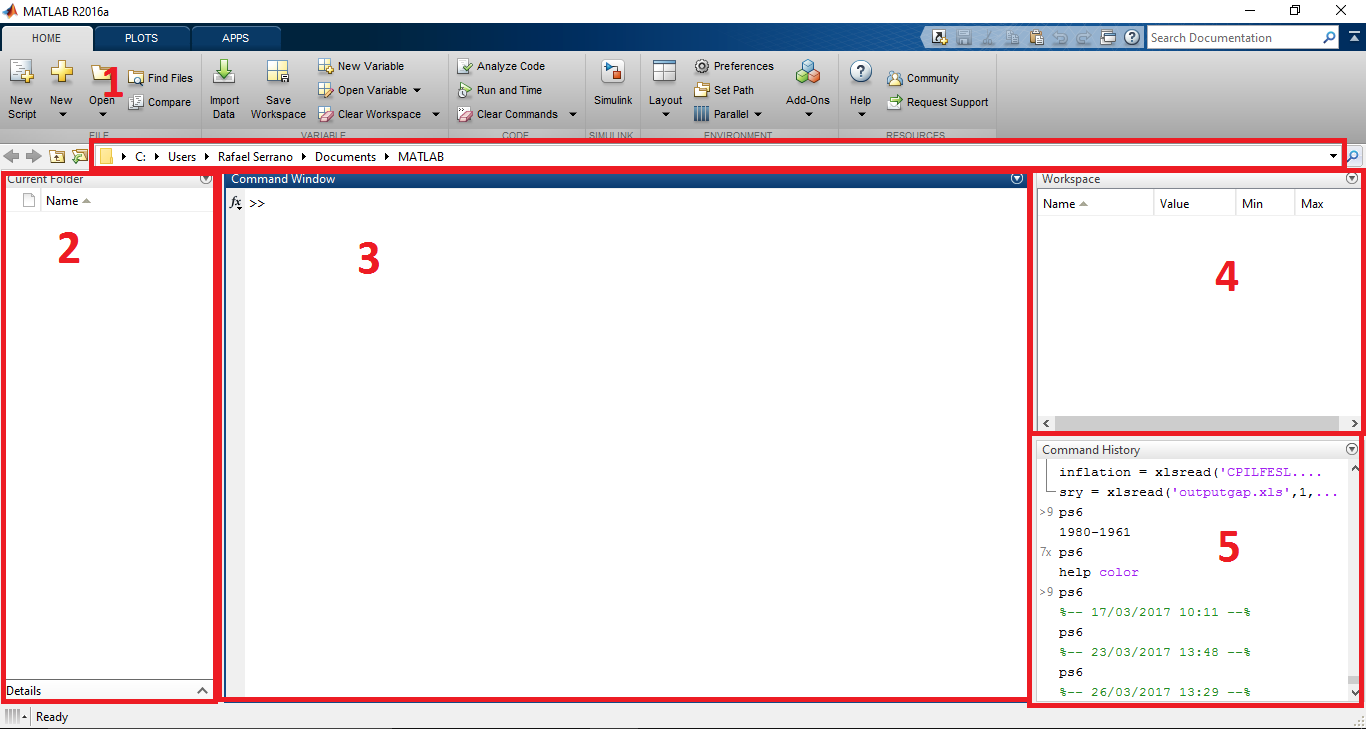
\includegraphics[width = 0.8\textwidth]{../figures/matlab_initial.PNG}
    \caption{Matlab's Interface}
    \label{fig:matlab_interface}
\end{figure}
\end{frame}

\section{Scripts vs Command Window}

\begin{frame}
    \frametitle{Scripts vs Commands}
\begin{itemize}
    \item The \alert{\textit{command window}} allows us to evaluate commands we type.
    \item \alert{\textit{Scripts}} are \textit{recipes} that can be saved. Useful for:
    \begin{itemize}
        \item Reproducing a set of codes \alert{exactly} in the same order
        \item Automating tasks
        \item Correcting mistakes in long tasks
    \end{itemize}
    \item A script is evaluated sequentially line by line.
\end{itemize}
\end{frame}

\begin{frame}[fragile]
    \frametitle{Scripts vs Commands}
    \begin{itemize}
        \item To start a new script:
        \begin{itemize}
            \item \verb;Home -> New Script;
            \item Type \verb;edit; in the command window
        \end{itemize}
        \item Write comments with the symbol \verb;%; 
        \item Everything after a \verb;%; will not be processed by Matlab
        \item A block of comments is defined within \verb;%{ %};
    \end{itemize}
\end{frame}

\begin{frame}[fragile]{Script Example}
\begin{lstlisting}
clear all
close all 
clc

% This is a comment

%{
    This is a block of comments. Everything within the two symbols is not processed by Matlab. Useful to define headers or helps for user defined functions.
%}
\end{lstlisting}
\end{frame}

\section{Creating Variables}

\begin{frame}
    \frametitle{Creating Variables}
    \begin{itemize}
        \item We can assign \textit{values} to a variable.
        \item Matlab has several types of objects (arrays, struct arrays, cell arrays...)
        \item To name a variable the first character \alert{\textbf{needs to be a letter}}.
        \item Matlab is case sensitive $x \neq X$
    \end{itemize}
\end{frame}

\begin{frame}[fragile]
    \frametitle{Creating Variables}
\alert{\textbf{Forbidden names:}}
\begin{itemize}
	\item $i$ and $j$ indicate complex numbers.
	\item \verb;pi; is assigned to $\pi$.
	\item \verb;ans; is assigned to the last value that has not been assigned to anything.
	\item \verb;Inf; or \verb;-Inf; are $\pm\infty$.
	\item \verb;NaN; represents \textit{``Not a Number''} (typically missing data).
	\item \verb;eps; is the \textit{machine epsilon} (we will comment a bit on this below).
\end{itemize}
\end{frame}

\begin{frame}[fragile]
    \frametitle{Creating Variables}
\begin{lstlisting}
clear
clc

%==========================================================
                % === Creating Variables === %
%==========================================================

% Assignment and basic operations
x = 5
x*2
x-7
x+7

% Creating variable from another
y = x^2;    % Semicolon ; suppresses output
disp(y)
\end{lstlisting}
\end{frame}

\begin{frame}[fragile]
    \frametitle{Matlab as a Calculator}
    \begin{itemize}
        \item To perform basic arithmetic operations Matlab uses five symbols.
        \item These operators are defined for both \alert{\textit{matrices and scalars}}.
    \end{itemize}
\begin{table}[htbp]
    \caption{Basic Arithmetic Operators}
    \label{tab:basic_operators}
    \begin{tabular}{@{}cl@{}}
    \toprule
    Operator & Meaning \\ \midrule
    \verb;+;  & Addition \\ 
    \verb;-;  & Subtraction \\ 
    \verb;*;  & Multiplication \\ 
    \verb;/;  & Division \\ 
    \verb;^;  & Exponentiation \\ \bottomrule
    \end{tabular}
\end{table}
\end{frame}

\begin{frame}
    \frametitle{Matlab as a Calculator}
\begin{exercise} 
    Use Matlab as a calculator and try to solve the following operations using the functions needed. Solve them for $x = 0$ and $x = \frac{\pi}{4}$
    
    \[
            \frac{\left(\ln\big( 1+x^2\big)\right)^2 - \sqrt{1+\sqrt[3]{x^2}\,}}{1+\sin^2 x} \ ; \  \ln\bigg\lvert\frac{x-\pi}{x+\pi}\bigg\rvert + \sqrt{\frac{e^x}{1+xe^x}}
    \]
\end{exercise}
\end{frame}

\begin{frame}[fragile]
    \frametitle{Matlab as a Calculator}
    Solving for $x = 0$. Check commands:
    \begin{itemize}
        \item \verb;log;, \verb;sqrt;, \verb;sin;, \verb;abs;, \verb;pi;
    \end{itemize}
\begin{lstlisting}
    % === Ex. 1: Solve Complex Operations === %
    x = 0;
    
    op1 = ((log(1+x^2))^2-sqrt(1+x^(2/3)))/(1+sin(x)^2);
    op2 = log(abs((x-pi)/(x+pi)))+sqrt(exp(x)/(1+x*exp(x)));
\end{lstlisting}
\end{frame}

\begin{frame}[fragile]
    \frametitle{Arrays --- Vectors and Matrices}
\begin{itemize}
    \item Matrices and arrays are the fundamental representation of data in Matlab.
    \item An \href{https://en.wikipedia.org/wiki/Array}{array} is just a systematic arrangement of objects. A vector is a one-dimensional array, while a matrix is a two-dimensional array.
    \item \alert{\textbf{Row vectors}} (the default in Matlab) are created as
\begin{lstlisting}
%=========================================================
                    % === Vectors === %
%=========================================================

rowV = [1 2 3 4 5];     % Spaces separate elements
rowV2 = [6,7,8,9,10];   % Commas work as spaces
\end{lstlisting}
\end{itemize}
\end{frame}

\begin{frame}[fragile]
    \frametitle{Arrays --- Vectors and Matrices}
\begin{itemize}
    \item \alert{\textbf{Column vectors}} are created with the semicolon operator \verb+;+
\begin{lstlisting}
colV = [1; 2; 3; 4; 5];
\end{lstlisting}
    \item Sequences as row vectors
\begin{lstlisting}
% A sequence from 0 to 10 in steps of 2
seq1 = 0:2:10;
% 1000 equally spaced elements in [0,10]
seq2 = linspace(0,10,1000);
\end{lstlisting}
    \item \alert{\textbf{Check your workspace!}}
\end{itemize}
\end{frame}

\begin{frame}[fragile]
    \frametitle{Arrays --- Vectors and Matrices}
\begin{itemize}
    \item \alert{\textbf{Matrices}} can be created element by element or by \textit{concatenating vectors}.
    \item A semicolon \verb+;+ after a number indicates a new row.
\begin{lstlisting}
A = [1 2 3; 4 5 6; 7 8 9];
B = [4 5 6; 7 9 2; 1 5 32];
ConcatenatedMatrix = [rowV;rowV2];
\end{lstlisting}
    \item Produces:
    \[
    A = \begin{bmatrix}
    1 & 2 & 3 \\
    4 & 5 & 6 \\
    7 & 8 & 9 
    \end{bmatrix} \ 
    B = \begin{bmatrix}
    4 & 5 & 6 \\
    7 & 9 & 2 \\
    1 & 5 & 32
    \end{bmatrix} \ 
    ConcatenatedMatrix = \begin{bmatrix}
    1 & 2 & 3 & 4 & 5 \\
    6 & 7 & 8 & 9 & 10
    \end{bmatrix}
    \]
\end{itemize}
\end{frame}

\begin{frame}[fragile]
    \frametitle{Arrays --- Vectors and Matrices}
\alert{\textbf{Array Indexing}}
    \begin{itemize}
        \item In matrix $A = \begin{bmatrix}
            1 & 2 & 3 \\
            4 & 5 & 6 \\
            7 & 8 & 9 
            \end{bmatrix}$ the element $a_{2,3} = 6$ is the element in row $2$ and column $3$.
        \item In Matlab we can access element $a_{j,k}$ as \verb;A(j,k); to access $6$ in matrix $A$ before:
\begin{lstlisting}
A(2,3)    % Element in row 2 and column 3 of matrix A
\end{lstlisting}
        \item For vectors, we can index by the position only.
\begin{lstlisting}
colV(1)   % First element in colV vector
\end{lstlisting}
    \end{itemize}
\end{frame}

\begin{frame}[fragile]
    \frametitle{Arrays --- Vectors and Matrices}
\alert{\textbf{Array Indexing}}
    \begin{itemize}
        \item For matrices in general, we can access whole columns or rows.
\begin{lstlisting}
A(2,:)      % Index the 2nd row and all columns
\end{lstlisting}
        \item In general, we can index matrices as
    \end{itemize}
    \begin{table}[htbp]
        \caption{Basic Indexing}
        \label{tab:basic_indexing}
        \begin{tabular}{@{}cl@{}}
        \toprule
        Index & Result \\ \midrule
        \verb+A(i,j)+  & $a_{i,j}$ \\ 
        \verb+A(i,:)+  & Row $i$ \\ 
        \verb+A(:,j)+  & Column $j$ \\ \bottomrule
        \end{tabular}
    \end{table}
\end{frame}

\begin{frame}[fragile]
    \frametitle{Arrays --- Operations}
    \begin{itemize}
        \item We can use the same operators described in Table \ref{tab:basic_operators} \alert{\textbf{BUT}} mind the laws of matrix algebra.
        \item Matrix products \verb+A*B+
        \[
        A = \begin{bmatrix}
            1 & 2 & 3 \\
            4 & 5 & 6 \\
            7 & 8 & 9 
            \end{bmatrix} \ 
        B = \begin{bmatrix}
            4 & 5 & 6 \\
            7 & 9 & 2 \\
            1 & 5 & 32
            \end{bmatrix}
        AB = \begin{bmatrix}
            21 & 38 & 106 \\
            57 & 95 & 226 \\
            93 & 152 & 346
        \end{bmatrix} 
        \]
        \item To transpose a matrix $A$:
\begin{lstlisting}
% To transpose a matrix use transpose() or '
A'
transpose(A)
\end{lstlisting}
    \end{itemize}
\end{frame}

\begin{frame}[fragile]
    \frametitle{Arrays --- Operations}
    \alert{\textbf{Element-wise Operations}}
\begin{itemize}
    \item Element-wise product of $A$ and $B$ is computed by $a_{i,j}\times b_{i,j}$
    \[
    A = \begin{bmatrix}
        1 & 2 & 3 \\
        4 & 5 & 6 \\
        7 & 8 & 9 
        \end{bmatrix} \ 
    B = \begin{bmatrix}
        4 & 5 & 6 \\
        7 & 9 & 2 \\
        1 & 5 & 32
        \end{bmatrix}
    A \odot B = 
    \begin{bmatrix}
        4  &  10 &   18 \\
        28  &  45 &   12 \\
        7  &  40 &  288
    \end{bmatrix}    
    \]
    \item In Matlab, we use
\begin{lstlisting}
% Element-wise multiplication of A and B
A.*B
    
% Be careful with element wise multiplication. Check what would happen if:
rowV.*rowV2'
\end{lstlisting}
\end{itemize}
\end{frame}

\begin{frame}[fragile]
    \frametitle{Arrays --- Matrix Operations}
    \begin{table}[htbp]
        \caption{Matrix Arithmetic Operations}
        \label{tab:matrix_operators}
        \begin{tabular}{@{}cl@{}}
        \toprule
        Operator & Meaning \\ \midrule
        \verb;+;  & Addition \\ 
        \verb;-;  & Subtraction \\ 
        \verb;*;  & Multiplication \\ 
        \verb;.*; & Element-wise product \\
        \verb;\;  & Left division $(A \setminus B = A^{-1}B)$. Equivalent to \verb;mldivide(); \\
        \verb;/;  & Right division $(A / B = AB^{-1})$. Equivalent to \verb;mrdivide(); \\
        \verb;./; & Element-wise division \\ 
        \verb;^;  & Exponentiation \\
        \verb;.^;  & Element-wise exponentiation \\
        \verb;inv(); & Inverse of matrix \\ \bottomrule
        \end{tabular}
    \end{table}
\end{frame}

\begin{frame}[fragile]
    \frametitle{Arrays --- Matrix Operations}
\begin{exercise} 
Solve the following system of linear equations using \verb;inv(); and \verb;\;.

\begin{alignat*}{7}
3x&& \; + \; &&2y&& \; - \; &&z&& \; = \; &&1&\\
2x&& \; - \; &&2y&& \; + \; &&4z&& \; = \; &&-2&\\
-x&& \; + \; &&{\tfrac {1}{2}}y&& \; - \; &&z&& \; = \; &&0&
\end{alignat*}
\end{exercise}
\end{frame}

\begin{frame}[fragile]
    \frametitle{Arrays --- Matrix Operations}
To solve systems of equations, it is recommended to use \verb;\; instead of \verb;inv();. If you're interested you can \href{https://www.mathworks.com/matlabcentral/answers/139778-what-is-the-difference-between-inv-and-the-backslash#answer_143286}{check this} or try \href{https://www.mathworks.com/help/matlab/ref/inv.html#bu6sfy8-1}{this example}.
\begin{lstlisting}
% === Ex.2 Solve the system === %
b = [1; - 2; 0];
A = [3 2 -1; 2 -2 4; -1 0.5 -1];
x = inv(A)*b;   % Slower and inaccurate
x_oth = A\b;    % This method is preferred
x_oth2 = mldivide(A,b); % Same as the previous one
disp([x,x_oth,x_oth2])
\end{lstlisting}
\end{frame}

\section{Relational and Logical Operators and Loops}

\begin{frame}
    \frametitle{Relational and Logical Operators}
    \alert{\textbf{Relational Operators}}
\begin{itemize}
    \item Check if $a\neq b$
    \item Check wether $a \lesseqgtr b$
\end{itemize}

\alert{\textbf{Logical Operators}}
\begin{itemize}
    \item Check wether one or more conditions are satisfied
    \item Access elements that are \textbf{NOT} equal to $a$.
\end{itemize}
\end{frame}

\begin{frame}
    \frametitle{Relational and Logical Operators}
\begin{itemize}
    \item Relational and logical operators return either \textit{true} or \textit{false} values.
    \item In Matlab, \textit{true} is coded with $1$ and \textit{false} with $0$.
    \item But \alert{\textbf{these are not numbers!!}}
    \item The result is a \textit{logical array}.
\end{itemize}
\end{frame}

\begin{frame}[fragile]
    \frametitle{Relational and Logical Operators}
\begin{lstlisting}
A > 5
A == 5
A <= 5
\end{lstlisting}

\begin{table}[htbp]
    \caption{Relational Operators}
    \label{tab:relational_operators}
    \begin{tabular}{@{}cl@{}}
    \toprule
    Operator & Meaning \\ \midrule
    \verb;==; & Exactly equal to \\
    \verb;~=; & NOT equal to \\
    \verb;<;  & Lower than \\
    \verb;<=; & Lower or equal than \\
    \verb;>;  & Lower than \\
    \verb;>=; & Lower or equal than \\ \bottomrule
    \end{tabular}
\end{table}
\end{frame}

\begin{frame}[fragile]
    \frametitle{Relational and Logical Operators}
\begin{lstlisting}
A > 5 | A < 9
~(A > 3 & A < 6)
\end{lstlisting}

\begin{table}[htbp]
    \caption{Logical Operators}
    \label{tab:logical_operators}
    \begin{tabular}{@{}cl@{}}
    \toprule
    Operator & Meaning \\ \midrule
    \verb;&; & Element-wise AND \\
    \verb;&&; & AND for scalars \\
    \verb;|;  & Element-wise OR \\
    \verb;||; & OR for scalars \\
    \verb;~;  & NOT \\ 
    \verb;any(); & True if any element of a vector is \textit{true} \\
    \verb;all(); & True if all elements of a vector are \textit{true} \\ \bottomrule
    \end{tabular}
\end{table}
\end{frame}

\begin{frame}[fragile]
    \frametitle{If-Else Statements}
    \begin{itemize}
        \item Typically, relational and logical operators are used as conditions.
        \item \alert{\textbf{If}} something happens, do something. \alert{\textbf{Else}} do another thing.
        \item If-Else statements start with \verb;if; and are closed with \verb;end;. General syntax:
    \end{itemize}
\begin{lstlisting}
b = 3;
if b < 0
    disp('b is negative')
else
    disp('b is non-negative')
end
\end{lstlisting}
\end{frame}

\begin{frame}[fragile]
    \frametitle{If-ElseIf-Else Statements}
\begin{itemize}
    \item If we want to include two possible conditions, we use \verb;elseif;
\end{itemize}
\begin{lstlisting}
b = 4;
if mod(b,2) == 0 % Check if even
    disp('b is even')
elseif mod(b,5) == 0 % Check if divisible by 5
    disp('b is divisible by 5')
else
    disp('b is not even nor divisible by 5')
end
\end{lstlisting}
\end{frame}

\begin{frame}[fragile]
    \frametitle{For and While Loops}
\begin{itemize}
    \item Sometimes we need to repeat the same operation several times.
    \item When we know how many times exactly, we should use \verb;for; loops.
    \item If we do not know how many times, but we know a criterion, then we should use \verb;while;
\end{itemize}
\end{frame}

\begin{frame}[fragile]
    \frametitle{For and While Loops}
Suppose we want to simulate an $AR(1)$ process for $100$ periods such as
\[
y_{t+1} = \rho y_t + \varepsilon_t
\]
where $\rho = 0.85,y_0 = 0$, and $\varepsilon_t \underset{iid}{\thicksim} \mathcal{N}(0,1)$

\begin{lstlisting}
T = 100;
rho = 0.85;
y = zeros(100,1);
for t=2:T
    y(t,1) = rho*y(t-1,1) + randn;
end
\end{lstlisting}
\alert{\textbf{Check command}} \verb;randn; \alert{\textbf{!!}}
\end{frame}

\begin{frame}[fragile]
    \frametitle{For and While Loops}
Suppose we want to add one to a number for as long as it remains below a threshold. We can use \verb;while; loops!
\begin{lstlisting}
a = 0;
while a < 25
    a = a + 1;
end
\end{lstlisting}
\end{frame}

\begin{frame}[fragile]
    \frametitle{An Example with Grades}
\begin{exercise}
Suppose we have a list of grades of students. Create a loop that goes through all the notes and checks whether that student has passed the subject or not. To get the list, generate a random list of 200 grades uniformly distributed between 0 and 10 (check \verb;rand; command), and to assign if a student has passed or not, generate a vector called \verb;passed; that equals one if the student has obtained a grade larger or equal than 5, and 0 otherwise.
\end{exercise}
\end{frame}

\begin{frame}[fragile]
    \frametitle{An Example with Grades}
\begin{lstlisting}
% === Ex. 5 List of students === %
nstudents = 200;
grades = 10.*rand(nstudents,1);
pass = ones(nstudents,1);
    
for student = 1:nstudents
    if grades(student,1) >= 5
        pass(student,1) = 1;
    else
        pass(student,1) = 0;
    end
end
\end{lstlisting}
\end{frame}

\begin{frame}[fragile]
    \frametitle{An Example with Grades --- A More Efficient Approach}
The previous example was perfectly correct, but we could improve performance by \alert{\textit{vectorizing}} the operations.

\begin{lstlisting}
pass_vect = zeros(nstudents,1);
pass_vect(grades >= 5) = 1;

% To test they are equal
isequal(pass,pass_vect)
\end{lstlisting}    

Vectorizing is \alert{\textbf{extremely important}}. In this simple example, the vectorized function takes $\approx 18\%$ of the time it takes for the loop.

\end{frame}

\section{Simple Plots}

\begin{frame}[fragile]
    \frametitle{Simple Plots}
    \begin{itemize}
        \item Matlab has a powerful command to generate figures \verb;plot;.
        \item To plot the $AR(1)$ process we simulated before, is as easy as
\begin{lstlisting}
figure
plot(1:T,y)
\end{lstlisting}
        \item Command \verb;figure; opens a clear figure window.
        \item \verb;plot; takes as first argument the $x-$axis vector (the time periods) and the value of $y_t$ as second argument.
    \end{itemize}
\end{frame}

\begin{frame}
    \frametitle{A More Involved Example}
\begin{figure}
    \centering
    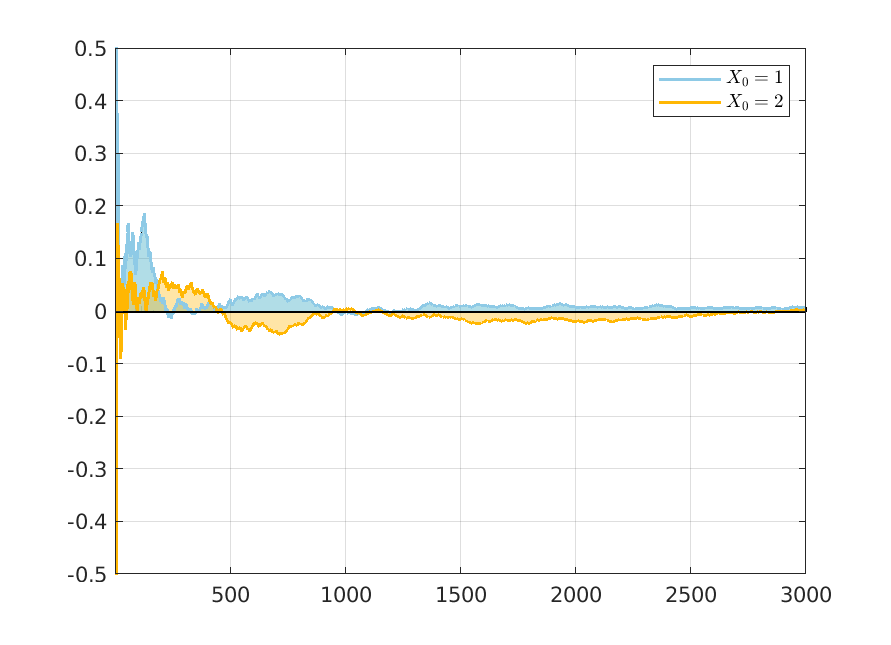
\includegraphics[width = 0.68\textwidth]{../figures/unemployment_dynamics.png}
    \caption{A Model of Unemployment Dynamics}
    \label{fig:unemployment}
\end{figure}
\end{frame}

\section{Functions}

\begin{frame}[fragile]
    \frametitle{User Defined Functions}
\begin{itemize}
    \item Commands are functions that take inputs and yield a result.
    \item In Matlab we can create our own functions just like in the mathematical sense.
    \item If $f(x) = 3x + 1$ then we can plug any $x$ and the result is $3x + 1$. This function in Matlab would be
\end{itemize}
\begin{lstlisting}
function [fx] = simple_function(x)
    fx = 3*x + 1;
end
\end{lstlisting}
\end{frame}

\begin{frame}[fragile]
    \frametitle{User Defined Functions}
\begin{itemize}
    \item The general structure of a function is
\begin{lstlisting}
function [out1,out2,...,outN] = name(in1,in2,...,inN)
    % Document the function. Author, inputs, outputs...
    Operations
    out1 = %operations to get out1;
    ...
    outN = %operations to get outN;
end
\end{lstlisting}
    \item Save the function as an \verb;.m; file in the working directory (or add to path).
    \item The name of the file \alert{\textbf{must be}} the name you assigned.
\end{itemize}
\end{frame}

\begin{frame}[fragile]
    \frametitle{User Defined Functions}
\begin{exercise}
Create a function called \verb;my_wave; that gives as output the plot of a sinusoidal wave. The function should take as arguments the parameters that will give the amplitude, the frequency, and the upper and lower bounds in which it will be plotted. By default, plot $1000$ points. Plot the sinusoidal wave with amplitude and frequency one for comparison. A sinusoidal wave $W$ with amplitude $A$ and frequency $f$ is computed as 
\[
W = A \sin(2\pi f x)
\]
\end{exercise}
\end{frame}

\begin{frame}[fragile]
    \frametitle{User Defined Functions}

A general function to compute a sine wave
\begin{lstlisting}
function [wave] = my_wave(A,freq,lb,ub)
    points = 1000;
    x = linspace(lb,ub,points);
    wave = A.*sin(2.*pi.*freq.*x);
    
    figure
    plot(x,wave,'--','LineWidth',1.3)
    hold on
    grid on
    plot(x,sin(x),'-','LineWidth',1.3)
    legend({'$A\sin(\omega x)$','$\sin(x)$'},'Interpreter','latex','Location','best')
    xlabel('$x$','Interpreter','latex')
    title(['Sinusoidal wave with amplitude ', num2str(A), ' and frequency ', num2str(freq)])
end
\end{lstlisting}
\end{frame}

\end{document}